\subsection{Introduction}

\subsubsection{Purpose}

This software requirements specification is intended to define the requirements of the 
project for developing a multi-camera, multispectral image processing system, that 
operates on an SoM at near real-time, for use in air based 
applications. Defined requirements will allow for a contract between us, the 
developers, and Rockwell Collins, our client, on what Rockwell Collins wants us to 
deliver in their desired software. This document is intended for review and reference 
by both the developers and the clients.\\

\subsubsection{Scope}

The product outlined in this requirements document will be the multi-camera, SoM based,
 near real-time video processing for UAS and VR/AR applications. This product will need to 
 be able to generate a stitched video output from a multi-camera input. The product is 
 intended to help initialize our client's development of a cheaper alternative to a 
 product that is currently offered to their customers.\\

The software products that will be produced include software for a stitched video output 
from the NVIDIA TX1/2, receiving the input from two visible band cameras. 
The video output is expected to be near real-time, and the latency from the camera 
input to the video output is expected to be improved upon throughout the project. Video 
output stretch goals are to have software that fuses the video output from the input of 
three, four, five, and six cameras; and to have up to four infrared band inputs.\\

Output display stretch goals will be to incorporate IMU data, orientation tracking 
data, GPS data, and geolocate imagery. Two final stretch goals are packaging the 
hardware for flight, and interfacing the system to support the client's desired 
cameras for input.\\

The goal of the software is to contribute to a project that will assist pilots during 
low visibility conditions during the day, night, and inclement weather for all phases 
of flight. The video input from infrared and visible band cameras combined with 
on-board sensor input, and databases will enhance a pilot's vision for a UAS.\\

\subsubsection{Definitions, Acronyms, Abbreviations}

\paragraph{Definitions}

\begin{tabular}{|l|p{11cm}|}
	\hline
	\textbf{Term} & \textbf{Definition}\\
	\hline
	geolocate imagery & image with associated location information.\\
	\hline
	low visibility & Inability to see clearly with the naked eye.\\
	\hline	
	multiple cameras & At least two cameras, but a maximum of six cameras for 
	video input.\\
	\hline
	near real-time & Fast enough that a human could not notice the time 
	delay (lag) between \newline real life images and images displayed by the system.\\
	\hline
	NVIDIA TX1/2 & NVIDIA GPUs, the Jetson TX1 or the Jetson TX2.\\
	\hline
	spectral bands & Electromagnetic frequency ranges; different 
	spectrums of light, including \newline but not limited to infrared 
	and visible light.\\
	\hline
	standalone & The system performs its functionality independent of another
	system, in our product's case it will be independent of a development kit. \\
	\hline
	stitched (video) output & a composite image formed from multiple images\\
	\hline
	time division multiplexing & The illusion of simultaneous execution in a CPU due
	to a CPU being capable of running one process at a time.\\
	\hline
\end{tabular}

\paragraph{Acronyms}

\begin{tabular}{|l|l|}
	\hline
	\textbf{Acronym} & \textbf{Term}\\
	\hline
	AR & Augmented Reality\\
	\hline
	CPU & Central Processing Unit\\
	\hline
	CSI & Camera Serial Interface\\
	\hline
	EVS & Enhanced Vision System\\
	\hline
	fps & Frames per second\\
	\hline
	GPS & Global Positioning System\\
	\hline
	GPU & Graphic Processing Unit\\
	\hline
	ISP & Image Signal Processors\\
	\hline
	IMU & Inertial Measurement Unit\\
	\hline
	HUD & Head-up Display\\
	\hline
	SoC & System-on-chip\\
	\hline
	SoM & System-on-module\\
	\hline
	SWaP-C & Size, weight, power and cost\\
	\hline
	UAS & Unmanned Aircraft System\\
	\hline
	VI & Video Input\\
	\hline
	VR & Virtual Reality\\
	\hline
\end{tabular}

\subsubsection{Overview}

This project aims to create a product that is capable of combining the video input from 
two or more cameras and produce an output at near real-time. Our proposed solution 
will use an NVIDIA Jetson TX1/2, which we will use for its integrated GPU and CPU.\\

We need this GPU to combine the images from multiple cameras. The end goal is to have 
a system that uses the input from multiple cameras that operate on the infrared and 
visible light spectral bands. By using these spectral bands, we should be able to 
produce an image that can be used to see in low-visibility situations, such as landing 
a UAS in fog.\\

The images we produce will be 2D representations of our collective image captures. In 
other words, we do not aim to create a 3D image or a dynamic focus image. This is 
certainly possible when using multiple cameras, but we simply aim to use multiple 
cameras on different spectral bands to create one image of one subject that is the 
combination of all images captured by the cameras.\\


\subsection{Overall Description}

\subsubsection{Product Perspective}

The system will be self-contained and consists of three parts: one NVIDIA TX1/2, 
one carrier board, and at least two cameras. The cameras connect to the carrier board, 
which is connected to the NVIDIA TX1/2. The NVIDIA TX1/2 is responsible for decoding 
the serial data retrieved by the CSI board from the cameras, and is then be used to 
execute the software for image processing and combining images from multiple cameras.\\

\begin{figure}[H]
	\centering
	\label{fig:ProductBlockDiagram}
	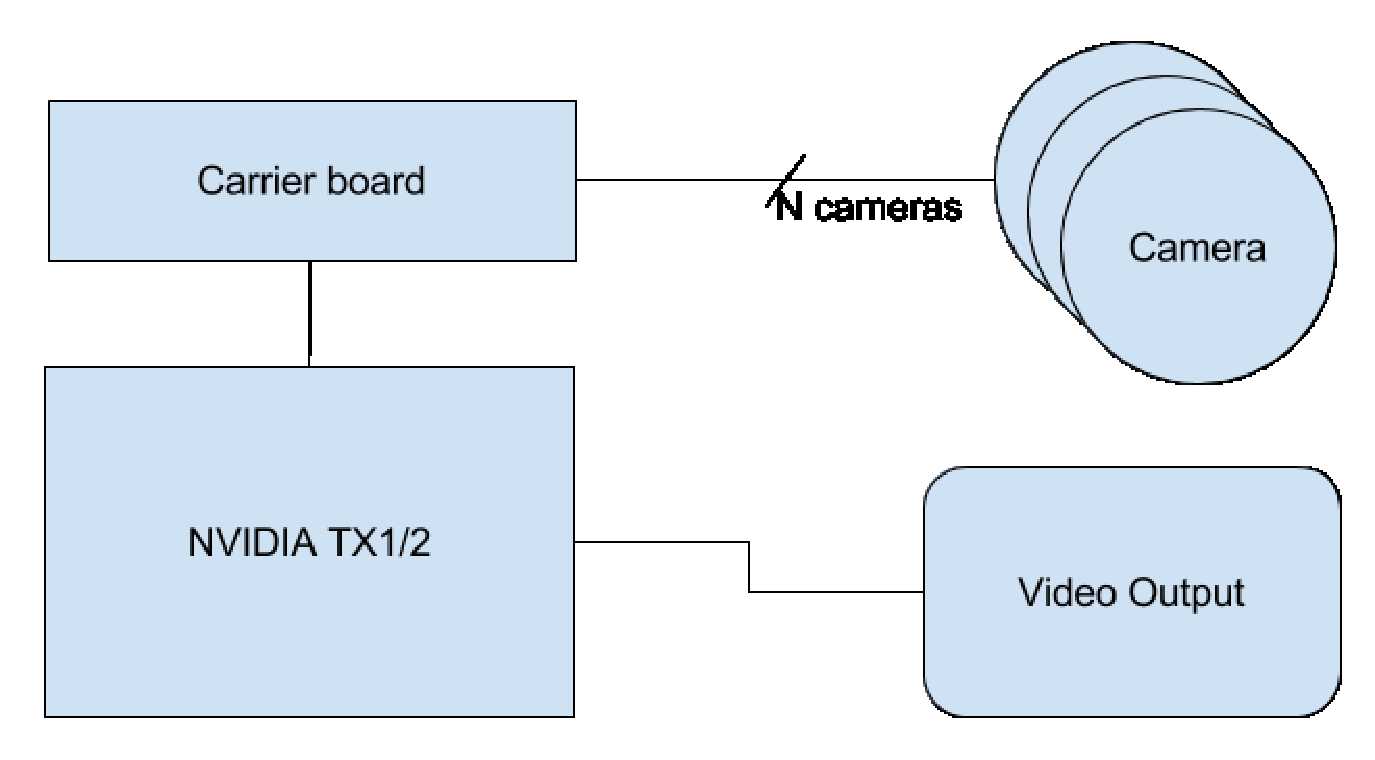
\includegraphics[width=10cm]{images/diagram.eps}
	\caption{Product Block Diagram \label{overflow}}
\end{figure}

\subsubsection{Product Functions}

The basic functionality of the product will be to produce stitched images on a video 
output that is provided by multiple camera inputs capable of sensing visible and 
infrared spectral bands. These images will be relayed in near real-time so that it 
can be used as a video feed for the pilot of a UAS during low visibility flight 
conditions. \\

A functional stretch goal for video output provided by camera input is to fuse the 
input from the visible and infrared spectral bands, which will overlay the two types of output 
and enhance the vision for a UAS pilot. \\

Output display functional stretch goals will be to provide indications from IMU data, 
orientation tracking data, GPS data, and geolocate imagery and have them displayed 
with the video output provided by the camera input. \\

\subsubsection{Constraints}

The client requires that the product's SoM be an NVIDIA TX1/2 to utilize its GPU 
and CSI ports. Due this product's application being on a UAS, its hardware must be 
compact to meet SWaP-C requirements set by the client. The system must be standalone 
and not rely on cloud computing and external databases. \\

The system must operate in near real-time, and therefore the video/camera feed(s) must be 
processed quickly enough for the user to be able to make snap decisions based on the feed. The 
NVIDIA TX1/2 should process each frame before the next one arrives to be processed. 
For example, when recording at 30 fps each output frame should be processed in 
less than 1/30 of a second.\\

\subsubsection{Assumptions \& Dependencies}

Software will be implemented on an NVIDIA TX1/2, and will be deployed with NVIDIA 
Jetpack software running on an Ubuntu machine. The NVIDIA TX1/2 is assumed to be 
capable of processing the data feed through its CSI interface. \\

Adequate power supplies are required; they should meet the NVIDIA TX1/2 system 
requirements. \\

All cameras in use should be aimed at same subject, capturing approximately the same 
image. Each camera should work independently of the system; if one fails, the others 
will still operate.\\

\subsection{Specific Requirements}

\subsubsection{Hardware Specifications}

\paragraph{NVIDIA Jetson TX1/2}

\begin{enumerate}[label=\alph*]
	\item The NVIDIA TX1/2 will receive image data through its CSI interface from
	the carrier board, and process this data to produce a video output. The carrier
	board is providing input to the NVIDIA TX1/2 from multiple cameras. \\
	\item The development environment of NVIDIA TX1/2 is available on the Ubuntu 
	operating system, and the module supports software for image processing.\\ 
	\end{enumerate}

\paragraph{Carrier Board}

\begin{enumerate}[label=\alph*]
	\item The carrier board should contain a CSI interface, which is used to transfer the
	input from up to six cameras to the NVIDIA TX1/2. \\
	\item The carrier board will provide output for a computer with data and signals that 
	can be used for subsequent image processing.\\
	\item The carrier board will be compatible with the NVIDIA TX1/2.\\
\end{enumerate}

\paragraph{Cameras}

\begin{enumerate}[label=\alph*]
	\item Cameras that use the CSI interface are required in order to transfer image data to 
	the NVIDIA TX1/2.\\
	\item The transfer rate is expected to operate at near real-time, and the output format 
	from the cameras will be accepted by NVIDIA TX1/2.\\
	\item The cameras should be able to capture images from different spectral bands 
	which includes infrared and visible light.\\
	\item The quality of the camera is not a primary concern for our project, and its 
	function is to is provide input to the NVIDIA TX1/2 for testing video output. 
	A stretch goal involves providing an interface to accomodate for cameras that 
	produces a higher quality input, but the hardware to connect these cameras to the 
	carrier board does not appear to exist at this time.\\
\end{enumerate}

\subsubsection{Software Specifications}

\begin{enumerate}[label=\alph*]
	\item The software running on the TX1/2 should be able to decode the data streams 
	from each camera and provide a stitched video output.\\
	\item The software should be able to stitch images from infrared 
	and visible light spectral bands to produce a 2D video output. \\
	\item Latency of the data-processing in the software is expected to be near 
	real-time, therefore the programming implemented will be required to use either time
	division multiplexing or parallel processing. \\
	\item The software stretch goals are to:
	\begin{enumerate}
	 	\item Output a dual stitched video combined with a fused six-camera input.\\
		\item Incorporate IMU data, orientation tracking data, GPS data, and geolocate 
		imagery into the video output. An IMU is used to track linear and angular 
		motion of an object by using gyroscopes and accelerometers. Orientation 
		tracking utilizes sensor input to provide rotational and position data.\\
		\item Provide an interface to accomodate for cameras the meet quality
		requirements for video output. \\
	\end{enumerate} 
\end{enumerate}

\subsection{Development Schedule}
	\begin{ganttchart}
    	[hgrid, x unit=0.77mm, y unit chart=9.0mm, title label font=\normalsize, time slot format=isodate]
    	{2017-11-01}{2018-05-31}
    	\gantttitlecalendar{year, month=name}\\
    	\ganttbar{Task 1}{2017-11-01}{2017-11-30}\\
    	\ganttbar{Task 2}{2017-11-15}{2018-01-06}\\
    	\ganttbar{Task 3}{2018-01-01}{2018-01-31}\\
    	\ganttbar{Task 4}{2018-01-15}{2018-02-28}\\
    	\ganttbar{Task 5}{2018-03-01}{2018-03-31}\\
    	\ganttbar{Task 6}{2018-04-01}{2018-04-30}\\
    	\ganttbar{Task 7}{2018-05-01}{2018-05-31}\\
    	\ganttlink{elem0}{elem1}
    	\ganttlink{elem1}{elem2}
    	\ganttlink{elem2}{elem3}
	\end{ganttchart}
\begin{center}
	Fig. 2: Project Schedule
\end{center}	

\subsubsection{Development Schedule Tasks}
Task 1: Have hardware procured and assembled when received.\\
Task 2: Produce stitched video output from the input of two and three cameras, 
and have latency estimates produced.\\
Task 3: Produce a tiled video output from the input of six cameras.\\
Task 4: Produce a dual stitched video output that is combined into a fused 
six-camera output (stretch goal).\\
Task 5: Incorporate IMU data, orientation tracking data, GPS data, and 
geolocate imagery into the video output (stretch goals).\\
Task 6: Package the system hardware for flight (stretch goal).\\
Task 7: Produce a software interface for the system to accomodate higher 
quality cameras (stretch goal).\\